\chapter{\bfseries Giếng Lượng Tử}
\label{Chapter4} %
Hàm sóng của điện tử trong giếng lượng tử có dạng sau:
\begin{equation}
\psi^{\alpha}(\mathbf{r})=\sum_{i=1}^{l_{\alpha}=14} F_i^{\alpha}(\mathbf{r})u_{i,k=0}(\mathbf{r})
\end{equation}
ở đây $u_{i,k=0}(\mathbf{r})$ là một hàm tuần hoàn với chu kỳ là hằng số mạng của tinh thể hệ số $\alpha=c,l_c=1\dots8$ tương ứng với vùng dẫn, $\alpha=v,l_v=9\dots 14$ tương ứng với vùng hóa trị  và $F_i^{\alpha}(\mathbf{r})$ là bao gồm tất cả các thành phần hàm envelope trong gần đúng envelope đôi khi người ta gọi là gần đúng khối lượng hiệu dụng ta có phương trình sau đây [8]:
\begin{equation}
\sum_{i=1}^{l_{\alpha}=14}\left[\mathcal{H}_{ij}^{\alpha}\left(-i\nabla\right) +V_i\left(\mathbf{r}\right)\delta_{ij}\right]F_i^{\alpha}(\mathbf{r})=E^{\alpha}F_j^{\alpha}(\mathbf{r})
\end{equation}
ở dây $H(\mathbf{k})$ là chuẩn Hamiltonian khối lượng hiệu dụng, $V_i\left(\mathbf{r}\right)$ là thế của giếng lượng tử nếu ta chọn trục lượng tử hóa theo trục $z\parallel[001]$ trong tinh thể thì ta có dạng sau, nói thêm thế $V_i\left(\mathbf{r}\right)$ có thể hiểu là khi 2 vật liệu đặt sát vào nhau thi sẽ có một lớp tiếp xúc giữa chúng có thể tại ra những điểm kỳ dị và dán đoạn của  dãy năng lượng và ta có thể tổng quát hóa nó thành một thế năng trong trường hợp này là thế năng của giếng lượng tử: 
\begin{align}
\mathcal{H}_{ij}^{\alpha}\left(-i\nabla\right)=\mathcal{H}_{ij}^{\alpha}\left(k_x,k_y,-i(\partial / \partial z)\right)=\mathcal{H}_{ij}^{\alpha}\left(k_{\parallel},-i(\partial / \partial z)\right)\notag \\
V_i\left(\mathbf{r}\right)=V_i\left(\mathbf{z}\right),\qquad F_j^{\alpha}(\mathbf{r})=e^{ik_{\parallel}r_{\parallel}}\Phi_i^{\alpha}(z)=e^{ik_xx}e^{ik_yy}\Phi_i^{\alpha}(z)
\end{align}
do đó ta viết lại phương trình trên lại như sau:
\begin{equation}
\sum_{i=1}^{14}\left[\mathcal{H}_{ij}^{\alpha}\left(k_{\parallel},-i(\partial / \partial z)\right) +V_i(\mathbf{r})\delta_{ij}\right]F_i^{\alpha ,k_{\parallel}}(\mathbf{r})=E^{\alpha ,k_{\parallel}}F_j^{\alpha ,k_{\parallel}}(\mathbf{r})
\end{equation}

Để giải phương trình (5.4) chúng ta cần phải tìm dạng của hàm envelope và điều kiện biên, một câu hỏi đặt ra điều kiện như thế nào là thích hợp ở đây tôi tham khảo [14,18]:
\begin{equation}
\hat{k}_zh(z)\longrightarrow -\frac{i}{2}\left(\frac{\partial}{\partial z}h(z) + h(z)\frac{\partial}{\partial z}\right), \qquad \hat{k}_z^2 \longrightarrow -\frac{\partial}{\partial z}h(z)\frac{\partial}{\partial z}
\end{equation}	  
còn hàm envelope có thể triển khai theo sóng phẳng như sau [6,7,8]
\begin{equation}
F_i^{\alpha,k_{\parallel}} = \sum_{l=1}^N a_{i,l}^{{\alpha},k_{\parallel}}\phi_l(z)
\end{equation}
với 
\begin{equation}
\phi_i\left(z\right) =  \begin{cases}
\sqrt{\frac{2}{L_z}}\sin\left[\frac{i\pi}{L_z}\left(z +\frac{L_z}{2}\right)\right] &\qquad\text{nếu} -\frac{L_z}{2}\le z\le \frac{L_z}{2}\\
0 &\qquad\text{các trường hợp còn lại}
\end{cases}
\end{equation}
ở đây $L_z$ là hằng số và nó thường được chọn sao cho lớn hơn nhiều lần so với bề dày của giếng lượng tử, thây biểu thức (5.6) vào (5.4) đồng thời nhân bên trái hai vế với đại lượng $\phi^{*}$ và chuẩn hóa nó theo $z$ ta có một hệ ma trận $14N\times 14N$
\begin{equation}
\sum_{i=1}^{14}\sum_{l=1}^{N}\langle \phi_{l} \vert \mathcal{H}_{ij} +V_i\delta_{ij}\vert \phi_{l^{'}} \rangle a_{il}^{\alpha,k_{\parallel}} = E^{\alpha,k_{\parallel}} a_{j
l^{'}}^{\alpha,k_{\parallel}}
\end{equation}
\section{Ứng dụng của giếng lượng tử}
Sau khi ta giải phương trình trên ta sẽ có cấu trúc năng lượng của chất bán dẫn trong giếng lượng tử, có các mức năng lượng ta có thể tính được nồng độ hạt tải của điện tử, lỗ trống, cũng như độ phân cực$\dots$ ta hãy xét Hamiltonian toàn phần của  hệ điện tử trong các dãy tương tác với ánh sáng (many-body system) có dạng sau [11,12,13,14,15]:   
\begin{equation}
\mathcal{H} = \mathcal{H}_{band \;structure} +\mathcal{H}_{light\;matter} +\mathcal{H}_{coulomb}
\end{equation}
trong đó $\mathcal{H}_{band\;structure}$ là Hamiltonian của hệ điện tử trong các dãy\footnote{Ở đây ta cần lưu ý rằng điệnt ử trong dãy hóa trị có phổ năng lượng âm, do đó nó cũng có một khối lượng $m_{\lambda=v <0}$, để tránh vấn đề khối lượng âm ta đưa ra khái niệm lổ trống như một giả hạt mới có điện tích dương và khối lương  $m_h= -m_v$. Sự tương đương về mặt vật lý của lổ trống và điện tử trong dãy hóa trị được giải thích như sau: Khi chưa có kích thích tất cả các điện tử trong chất bán dẫn sẽ lấp đầy tất cả các mức năng lượng của hóa trị, khi có kích thích một điện tử ở vùng hóa trị sẽ nhãy lên vùng dẫn và để lại trong dãy hóa trị một chỗ trống trong phổ năng lượng gây ra bởi quá trình hấp thụ lấp-bỏ chổ trống giữa các điện tử ở vùng hóa trị còn lại, có nghĩa là một điện tử ở vùng hóa trị bất kỳ sẽ có khả năng bỏ vị trí lấp đầy của nó để lấp đầy chổ trống vừa được tạo ra bởi một điện tử khác, lập lại quá trình đối với lỗ trống mới $\dots$ Và như vậy ta có một quá trình song song giửa chổ trống và các điện tử hóa trị, khi đó ta dồng nhất vai trò của một điện tử hóa trị bằng khái niệm lổ trống với tư cách là giả hạt mô tả chuyển dộng của chổ trống năng lượng trong dãy hóa trị Sự tương phản giửa lổ trống và điện tử ở vùng hóa trị cho phép ta xem lỗ trống như một giả hạt thật sự với khối lượng dương, điện tích dương. trong điều kiện cân bằng xác xuất để tìm thấy một lổ trống trong trạng thái k được cho bởi 
\(n_{h,k}= 1-n_{v,k}\) , có nghĩa là việc tìm thấy một lổ trống ở trạng thái k đồng nghĩa với việc mất đi một điện tử hóa trị trong trạng thái tương ứng },$\mathcal{H}_{light\;matter}$ là Hamiltonian tương ứng với tương tác của điện tử với trường ngoài và $\mathcal{H}_{coulomb}$ là Hamiltonian của thế Coulomb, trong  biễu diễn lượng tử hóa lần hai chúng có dạng sau đây:
\begin{align}
\mathcal{H}_{band\;structure} &= \sum_{\lambda,k_{\parallel}}E_{k_{\parallel}}^{\lambda}a_{\lambda k_{\parallel}}^{\dagger}a_{\lambda k_{\parallel}}\notag\\
\mathcal{H}_{light\;matter} &= \frac{e}{m_0}\mathcal{A}(t)P=\frac{e}{m_0}\mathcal{A}(t)\sum_{\lambda\lambda^{'}k_{\parallel}}\Pi_{k_{\parallel}}^{\lambda\lambda^{'}}
a_{\lambda k_{\parallel}}^{\dagger}a_{\lambda k_{\parallel}}
\end{align} 
chú ý ở trên ta đâ bỏ đi số hạng $\frac{e\mathcal{A}^2}{2m}$ xem [15,16] hoặc ở phụ lục, ở đây $\mathcal{A}(t)$ là thế véctơ của trường ánh sáng,$a_{\lambda k_{\parallel}}^{\dagger},a_{\lambda k_{\parallel}}$  lần lượt là toán tử sinh và  toán tử hủy, $\Pi_{k_{\parallel}}^{\lambda\lambda^{'}}$ là thành phần ma trận động lượng trong trường hợp này là ma trận động lượng $14\times14$ kp và nó có giá trị sau đây
\begin{equation}
\Pi_{k_{\parallel}}^{\lambda\lambda^{'}} = \int dz\sum_{nm}f_{nk_{\parallel}}^{\lambda *}(z)\pi_{nm}(k_{\parallel},-i\partial
_z)f_{mk_{\parallel}}^{\lambda^{'}}(z)
\end{equation}
với $\pi_{nm}=\frac{m_0}{\hbar}P_{nm}=\frac{m_0}{\hbar}\nabla_{k}\mathcal{H}_{nm}(k)$ và ta cần chú rằng $\mathcal{H}\propto\frac{e}{m_0}\mathcal{A}\mathbf{P}\propto\mathbf{r}\mathbf{E}$ do đó ta có thể biểu diễn $\mathcal{H}_{light\;matter}$ theo thế véctơ hoặc điện trường trong bài báo cáo này tôi sử dụng thế véctơ, còn thành phần Hamiltonian Coulomb trong multi-subband giếng lượng tử có dạng sau đây:
\begin{equation}
\mathcal{H}_{Coulomb}= \frac{1}{2}\sum_{\lambda_1\lambda_2\lambda_3\lambda_4 k_{\parallel}k_{\parallel}^{'}q_{\parallel}}
V_{k_{\parallel}k_{\parallel}^{'}q_{\parallel}}^{\lambda_1\lambda_2\lambda_3\lambda_4}
\times a_{\lambda_1 k_{\parallel} +q_{\parallel}}^{\dagger}a_{\lambda_2 k_{\parallel}^{'}-q_{\parallel}}^{\dagger}a_{\lambda_3 k_{\parallel}^{'}}a_{\lambda_4 k_{\parallel}}
\end{equation}
ở đây thành phần ma trận thế Coulomb thuộc nhiều dãy trong giếng lượng tử được cho bởi dạng sau [17]
\begin{equation}
V_{k_{\parallel}k_{\parallel}^{'}q_{\parallel}}^{\lambda_1\lambda_2\lambda_3\lambda_4}
=\frac{e^2}{2\epsilon\epsilon_0 L^2|q_{\parallel}|}\int dz_1\int dz_2
e^{-|q_{\parallel}||z_2-z_1|}\times\sum_{m} f_{mk_{\parallel}+q_{\parallel}}^{\lambda_1 *}(z_1)
f_{mk_{\parallel}}^{\lambda_4}(z_1)
\sum_{n}f_{nk_{\parallel}^{'}-q_{\parallel}}^{\lambda_2 *}(z_2)
f_{nk_{\parallel}^{'}}^{\lambda_3}(z_2) 
\end{equation}
để dẫn ra phương trình chuyển động cho hàm phân bố điện tử, lổ trống và hàm phân cực (thể hiện mối tương quan giữa cặp điện tử ở vùng dẫn và lổ trống ở vùng hóa trị), ta sử dụng phương trình chuyển động của các toán tử của Heisenberg sau đó ta lấy trị trung bình ta sẽ có kết quả cần tìm, ta hãy tìm nó thử xem có đạng như thế nào, như ta đã biết phương trình chuyển động Heisenberg có dạng sau:
\begin{equation}
\frac{d}{dt}\langle \mathcal{A}\rangle = \frac{i}{\hbar}\langle[\mathcal{H},\mathcal{A}]\rangle
\end{equation}
dấu $\langle\rangle$ được hiểu là lấy trị trung bình, ta xét đại lượng sau $\chi_{k_{\parallel}}^{\lambda\lambda^{'}}=\langle a_{\lambda k_{\parallel}}^{\dagger}a_{\lambda^{'} k_{\parallel}}\rangle$, ở đây $\lambda,\lambda^{'}$ lần lượt là chỉ số $c,c^{'}$ nếu ở vùng dẫn, $v,v^{'}$ nếu ở vùng hóa trị , nếu ta xét trường hợp $\lambda=\lambda^{'}$ thì ta sẽ có các đại lượng như $n_{k_{\parallel}}^{c} = \langle a_c^{\dagger}a_c\rangle,n_{k_{\parallel}}^{v} = \langle a_v^{\dagger}a_v\rangle$ tương ứng là nồng độ hạt tải của điện tử và lỗ trống và nó thể hiện tính chất dẫn điện, nếu ta xét trường hợp $\lambda\neq\lambda^{'}$ thì ta cũng có các đại lượng $n_{k_{\parallel}}^{cc^{'}} = \langle a_c^{\dagger}a_{c^{'}}\rangle,n_{k_{\parallel}}^{vv^{'}} = \langle a_v^{\dagger}a_{v^{'}}\rangle$ cho biết thông tin tương quan của hai dãy dẫn hoặc hai dãy hóa trị kề cận với nhau, còn đại lượng $\rho^{vc}$ là đại lượng phân cực thể hiện mối tương quan giữa điện tử và lỗ trống.\\
Khi tính toán với các toán tử sinh, hủy ta sử dụng các hệ thức sau đây:
\begin{align}
&[a_i,a_j^{\dagger}]= \delta_{ij},\qquad[a_i,a_j]=[a_i^{\dagger},a_j^{\dagger}]=0 \qquad (boson)\notag\\
&\{a_i,a_j^{\dagger}\}= \delta_{ij},\qquad \{a_i,a_j\}=\{a_i^{\dagger},a_j^{\dagger}\}=0 \qquad (fermion)\notag\\
&[b_v^{\dagger}b_v,b_r] =-b_v\delta_{vr},\qquad [b_v^{\dagger}b_v,b_r^{\dagger}]=b_v^{\dagger}\delta_{vr}\notag\\
&[AB,C]=A[B,C] +[A,C]B,\notag\\
&[A,BC]=[A,B]C+B[A,C],\notag\\
&[AB,C]=A\{B,C\}-\{A,C\}B
\end{align}
thây biểu thức Hamiltonian (5.9) và $\chi_{k_{\parallel}}^{\lambda\lambda^{'}}=\langle a_{\lambda k_{\parallel}}^{\dagger}a_{\lambda^{'} k_{\parallel}}\rangle$ vào phương trình chuyển động (5.14) ta có
\begin{equation}
\frac{\partial}{\partial t}\chi_{k_{\parallel}}^{\lambda\lambda^{'}} =\frac{i}{\hbar}\langle[\mathcal{H}_{band \;structure} +\mathcal{H}_{light\;matter} +\mathcal{H}_{coulomb},a_{\lambda k_{\parallel}}^{\dagger}a_{\lambda^{'} k_{\parallel}^{'}}]\rangle
\end{equation}
xét số hạng thứ nhất 
\begin{align}
&\frac{i}{\hbar}\biggl[\mathcal{H}_{band \;structure},a_{\lambda k_{\parallel}}^{\dagger}a_{\lambda^{'} k_{\parallel}^{'}}\biggr]=\frac{i}{\hbar}\sum_{\mu k_{\parallel}}E_{k_{\parallel}}^{\mu}\biggl[a_{\mu k_{\parallel}}^{\dagger}a_{\mu k_{\parallel}},a_{\lambda k_{\parallel}}^{\dagger}a_{\lambda^{'} k_{\parallel}^{'}}\biggr]\notag\\
&=\frac{i}{\hbar} \sum_{\mu k_{\parallel}}E_{k_{\parallel}}^{\mu}
\left(\biggl[a_{\mu k_{\parallel}}^{\dagger}a_{\mu k_{\parallel}},a_{\lambda k_{\parallel}}^{\dagger}\biggr]a_{\lambda^{'} k_{\parallel}^{'}}
+a_{\lambda k_{\parallel}}^{\dagger}\biggl[a_{\mu k_{\parallel}}^{\dagger}a_{\mu k_{\parallel}},a_{\lambda^{'} k_{\parallel}^{'}}
\biggr] \right)\notag\\
&=\frac{i}{\hbar} \sum_{\mu k_{\parallel}}E_{k_{\parallel}}^{\mu}\left(
\delta_{\mu\lambda}\delta_{k_{\parallel}k_{\parallel}} a_{\mu k_{\parallel}}^{\dagger}a_{\lambda^{'}k_{\parallel}^{'}}
-\delta_{\mu \lambda^{'}}\delta_{k_{\parallel}k_{\parallel}^{'}}a_{\lambda k_{\parallel}}^{\dagger}a_{\mu k_{\parallel}^{'}}
\right)\notag\\
&=\frac{i}{\hbar}\left( \underbrace
{\sum_{\mu k_{\parallel}}E_{k_{\parallel}}^{\mu}
\delta_{\mu\lambda}\delta_{k_{\parallel}k_{\parallel}}a_{\mu k_{\parallel}}^{\dagger}a_{\lambda^{'}k_{\parallel}^{'}}}_{\mu =\lambda}
- \underbrace{\sum_{\mu k_{\parallel}}E_{k_{\parallel}}^{\mu}\delta_{\mu \lambda^{'}}\delta_{k_{\parallel}k_{\parallel}^{'}}a_{\lambda k_{\parallel}}^{\dagger}a_{\mu k_{\parallel}^{'}}}_{\mu=\lambda^{'},k_{\parallel}=k_{\parallel}^{'}}
\right)\notag\\
&=\frac{i}{\hbar} \left(E_{k_{\parallel}}^{\lambda}
 a_{\lambda k_{\parallel}}^{\dagger}a_{\lambda^{'}k_{\parallel}}
-E_{k_{\parallel}}^{\lambda^{'}} a_{\lambda k_{\parallel}}^{\dagger}a_{\lambda^{'} k_{\parallel}}
\right) = \frac{i}{\hbar} a_{\lambda k_{\parallel}}^{\dagger}a_{\lambda^{'} k_{\parallel}}\left(E_{k_{\parallel}}^{\lambda}-E_{k_{\parallel}}^{\lambda^{'}} \right)
\end{align}
xét số hạng thứ hai
\begin{align}
&\frac{i}{\hbar}\biggl[\mathcal{H}_{light \;matter},a_{\lambda k_{\parallel}}^{\dagger}a_{\lambda^{'} k_{\parallel}^{'}}\biggr]=\frac{i}{\hbar}\frac{e}{m_0}\mathcal{A}(t)\sum_{\mu\mu^{'}k_{\parallel}}\Pi_{k{\parallel}}^{\mu\mu^{'}}
\biggl[
a_{\mu k_{\parallel}}^{\dagger}a_{\mu^{'} k_{\parallel}},a_{\lambda k_{\parallel}}^{\dagger}a_{\lambda^{'} k_{\parallel}^{'}}\biggr]\notag\\
&=\frac{i}{\hbar}\frac{e}{m_0}\mathcal{A}(t)\sum_{\mu\mu^{'}k_{\parallel}}\Pi_{k{\parallel}}^{\mu\mu^{'}}
\biggl[a_{\mu k_{\parallel}}^{\dagger}a_{\mu^{'} k_{\parallel}},a_{\lambda k_{\parallel}}^{\dagger}\biggr]a_{\lambda^{'} k_{\parallel}^{'}} + 
a_{\lambda k_{\parallel}}^{\dagger}\biggl[a_{\mu k_{\parallel}}^{\dagger}a_{\mu^{'} k_{\parallel}},a_{\lambda^{'} k_{\parallel}^{'}}\biggr]\notag\\
&=\frac{i}{\hbar}\frac{e}{m_0}\mathcal{A}(t)\sum_{\mu\mu^{'}k_{\parallel}}\Pi_{k{\parallel}}^{\mu\mu^{'}}
\left(
a_{\mu k_{\parallel}}^{\dagger}\{a_{\mu^{'} k_{\parallel}},a_{\lambda k_{\parallel}}^{\dagger}\}a_{\lambda^{'}k_{\parallel}^{'}}-
a_{\lambda k_{\parallel}}^{\dagger}\{a_{\mu k_{\parallel}}^{\dagger}a_{\lambda^{'}k_{\parallel}^{'}}\}a_{\mu^{'} k_{\parallel}}
\right)\notag\\
&=\frac{i}{\hbar}\frac{e}{m_0}\mathcal{A}(t)\sum_{\mu\mu^{'}k_{\parallel}}\Pi_{k{\parallel}}^{\mu\mu^{'}}
\left(
a_{\mu k_{\parallel}}^{\dagger}a_{\lambda^{'}k_{\parallel}^{'}}\delta_{\mu^{'}\lambda}
\delta_{k_{\parallel}k_{\parallel}} -
a_{\lambda k_{\parallel}}^{\dagger}a_{\mu^{'} k_{\parallel}}\delta_{\lambda^{'}\mu}\delta_{k_{\parallel}k_{\parallel}^{'}}
\right)\notag\\
&=\frac{i}{\hbar}\frac{e}{m_0}\mathcal{A}(t)\sum_{\mu k_{\parallel}}\Pi_{k{\parallel}}^{\mu\lambda}a_{\mu k_{\parallel}}^{\dagger}a_{\lambda^{'}k_{\parallel}}
-\frac{i}{\hbar}\frac{e}{m_0}\mathcal{A}(t)\sum_{\mu^{'}k_{\parallel}}\Pi_{k{\parallel}}^{\lambda^{'}\mu^{'}}
a_{\lambda k_{\parallel}}^{\dagger}a_{\mu^{'} k_{\parallel}}\notag\\
&=\frac{i}{\hbar}\frac{e}{m_0}\mathcal{A}(t)\sum_{\mu k_{\parallel}}\Pi_{k{\parallel}}^{\mu\lambda}a_{\mu k_{\parallel}}^{\dagger}a_{\lambda^{'}k_{\parallel}}
-\frac{i}{\hbar}\frac{e}{m_0}\mathcal{A}(t)\sum_{\mu k_{\parallel}}\Pi_{k{\parallel}}^{\lambda^{'}\mu}
a_{\lambda k_{\parallel}}^{\dagger}a_{\mu k_{\parallel}}\notag\\
&=\frac{i}{\hbar}\frac{e}{m_0}\mathcal{A}(t)\sum_{\mu k_{\parallel}}\Pi_{k{\parallel}}^{\mu\lambda}\chi_{k_\parallel}^{\mu\lambda^{'}}
-\frac{i}{\hbar}\frac{e}{m_0}\mathcal{A}(t)\sum_{\mu k_{\parallel}}\Pi_{k{\parallel}}^{\lambda^{'}\mu}
\chi_{k_{\parallel}}^{\lambda\mu}
\end{align}
số hạng tương tác thế Coulomb còn lại ta tính tương tự và chú ý rằng ta sẽ sử dụng kết quả gần đúng ở mục (2.9) ta có số hạng thứ ba như sau:
\begin{align}
\frac{i}{\hbar}\biggl[\mathcal{H}_{Coulomb},a_{\lambda k_{\parallel}}^{\dagger}a_{\lambda^{'} k_{\parallel}^{'}}\biggr]
&=\frac{i}{\hbar}\frac{e}{m_0}\sum_{\mu\mu_1\nu q}
V_{k_{\parallel}}^{\mu_1\lambda^{'}\nu\mu}\chi_{k_{\parallel}+q_{\parallel}}
^{\mu_1\nu}\chi_{k_{\parallel}}^{\lambda\mu}\notag\\
&- \frac{i}{\hbar}\frac{e}{m_0}\sum_{\mu\mu_1\nu q}
V_{k_{\parallel}}^{\mu_1\mu\nu\lambda}\chi_{k_{\parallel}+q_{\parallel}}
^{\mu_1\nu}\chi_{k_{\parallel}}^{\mu\lambda^{'}}
+\frac{\partial}{\partial t}\chi_{k_{\parallel}}^{\lambda\lambda^{'}}\Bigl\vert_{coll}
\end{align}
thây các giá trị (5.17),(5.18),(5.19) vào phương trình (5.16) ta có dạng tổng quát sau đây:
\begin{align}
\frac{\partial}{\partial t}\chi_{k_{\parallel}}^{\lambda\lambda^{'}}=
\frac{i}{\hbar}\left(E_{k_{\parallel}}^{\lambda} - E_{k_{\parallel}}^{\lambda^{'}}\right)\chi_{k_{\parallel}}^{\lambda\lambda^{'}} +\frac{i}{\hbar}\sum_{\mu}
\left[
\Omega_{k_{\parallel}}^{\mu\lambda}\chi_{k_{\parallel}}^{\mu\lambda^{'}} -
\Omega_{k_{\parallel}}^{\lambda^{'}\mu}\chi_{k_{\parallel}}^{\lambda\mu}
\right]
+\frac{\partial}{\partial t}\chi_{k_{\parallel}}^{\lambda\lambda^{'}}\Bigl\vert_{coll}
\end{align}	
trong đó 
\begin{equation}
\Omega_{k_{\parallel}}^{\lambda\lambda^{'}}=\frac{e}{m_0}\mathcal{A}(t).\Pi_{k_{\parallel}}^{\lambda\lambda^{'}} -\sum_{\mu\nu q_{\parallel}}
V_{k_{\parallel},k_{\parallel}+q_{\parallel},q_{\parallel}}^{\mu\lambda\nu\lambda^{'}}
\chi_{k_{\parallel}+q_{\parallel}}^{\mu\nu}
\end{equation}
khi $\lambda\neq\lambda^{'}$ thì đại lượng $\Omega_{k_{\parallel}}^{\lambda\lambda^{'}}$ được gọi là tần số tái chuẩn hóa Rabi, còn khi $\lambda = \lambda^{'}$ được gọi là năng lượng chuẩn hóa của dãy năng lượng và đại lượng $\frac{\partial}{\partial t}\chi_{k_{\parallel}}^{\lambda\lambda^{'}}\Bigl\vert_{coll}$ 	được gọi là số hạng mô tả qua chạm hoặc tán xạ được tính gần đúng trong thời gian khử pha.
\begin{figure}[hc]
\centering
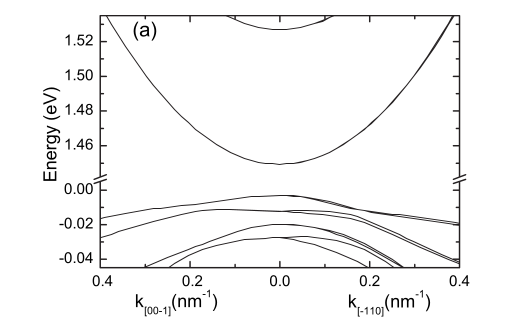
\includegraphics[width=0.70\textwidth]{./Figures/well1.png}
\caption[cấu trúc vùng năng lượng trong quantum well]{Cấu trúc vùng năng lượng của chất bán dẫn $GaAs/Al_{0.35}Ga_{0.65}As$ trong giếng lượng tử với bờ rộng là 12.nm với trục $k_{[110]}$ Ref[16]}
\end{figure}
\section{Dòng spin và dòng điện tích}
Sau khi giải phương trình trên ta sẽ có các đại lượng $n_{k_{\parallel}}^{cc},n_{k_{\parallel}}^{vv}$ tương ứng với nồng độ (mật độ)  hạt tải của điện tử và lổ trống (population), còn các đại lượng $n_{k_{\parallel}}^{cc^{'}},n_{k_{\parallel}}^{vv^{'}}$ cũng thể hiện mối tương quan của 2 dãy kề cận với nhau (intersubband coherences) và cuối cùng là đại lượng $\rho_{k_\parallel}^{cv}$ là đại lượng phân cực thể hiện mối tương quan của điện tử và lổ trống. Như ta đã biết dòng điện được định nghĩ như sau:
\begin{equation}
\mathbf{J}^{pop}(t) =nqv=\frac{e}{m_0}\sum_{c,k_{\parallel}}\Pi_{k_{\parallel}}^{cc}n_{k_{\parallel}}^{cc} +
\frac{e}{m_0}\sum_{v,k_{\parallel}}\Pi_{k_{\parallel}}^{vv}n_{k_{\parallel}}^{vv}
\end{equation}
dòng này tôi gọi là dòng population, còn dòng intersubband coherences được định nghĩa như sau:
\begin{equation}
\mathbf{J}^{coh}(t) =nqv=\frac{e}{m_0}\sum_{c\neq c^{'},k_{\parallel}}\Pi_{k_{\parallel}}^{cc^{'}}n_{k_{\parallel}}^{cc^{'}} +
\frac{e}{m_0}\sum_{v\neq v^{'},k_{\parallel}}\Pi_{k_{\parallel}}^{vv^{'}}n_{k_{\parallel}}^{vv^{'}}
\end{equation}
Tương tự ta định nghĩa dòng spin population và spin coherent như sau theo hướng $i=x,y,z$, ta có dòng spin population như sau: 
\begin{equation}
\mathbf{S}^{pop}(t) = \frac{\hbar}{m_0}\sum_{c,\mathbf{k}_\parallel}
{\displaystyle\mathsmaller{\mathsmaller{\sum\nolimits_{i\mathbf{k}_\parallel}^{cc}}}}
\Pi_{k_{\parallel}}^{cc}n_{k_{\parallel}}^{cc} +
\frac{\hbar}{m_0}\sum_{v,\mathbf{k}_\parallel}
{\displaystyle\mathsmaller{\mathsmaller{\sum\nolimits_{i\mathbf{k}_\parallel}^{vv}}}}
\Pi_{k_{\parallel}}^{vv}n_{k_{\parallel}}^{vv}
\end{equation}
và dòng spin coherent như sau:
\begin{equation}
\mathbf{S}^{coh}(t) = \frac{\hbar}{m_0}\sum_{c\neq c^{'},\mathbf{k}_\parallel}
{\displaystyle\mathsmaller{\mathsmaller{\sum\nolimits_{i\mathbf{k}_\parallel}^{cc^{'}}}}}
\Pi_{k_{\parallel}}^{cc^{'}}n_{k_{\parallel}}^{cc^{'}} +
\frac{\hbar}{m_0}\sum_{v\neq v^{'},\mathbf{k}_\parallel}
{\displaystyle\mathsmaller{\mathsmaller{\sum\nolimits_{i\mathbf{k}_\parallel}^{vv^{'}}}}}
\Pi_{k_{\parallel}}^{vv^{'}}n_{k_{\parallel}}^{vv^{'}}
\end{equation}
hình chiếu thành phần i của spin lên các trục $x,y,z$ được miêu tả bởi thành phần ma trận mômen động lượng như sau [22,16]:
\begin{equation}
{\mathsmaller{\sum\nolimits_{i\mathbf{k}_\parallel}^{cc^{'}}}} =
\frac{1}{2}\int dz\sum_{mn}
f_{m\mathbf{k}_{\parallel}}^{c*}(z)
\boldsymbol{\sigma}_i
f_{n\mathbf{k}_{\parallel}}^{c^{'}}(z)
\end{equation}
và 
\begin{equation}
{\mathsmaller{\sum\nolimits_{i\mathbf{k}_\parallel}^{vv^{'}}}} =
\frac{1}{2}\int dz\sum_{mn}
f_{m\mathbf{k}_{\parallel}}^{v*}(z)
\boldsymbol{\mathcal{J}}_i
f_{n\mathbf{k}_{\parallel}}^{v^{'}}(z)
\end{equation}
ở đây $\boldsymbol{\sigma}_i$ là ma trận Pauli, còn $\boldsymbol{\mathcal{J}}_i$ là ma trận với spin bằng $j=-3/2$. sau khi ta có các đại lượng dòng spin và dòng điện tích của các trường hợp coherent và population ta định nghĩa đại lượng tổng của hai dòng này như:\\
Tổng dòng điện tích của điện tử hoặc lổ trống đống góp vào dòng injection như sau:
\begin{equation}
\mathbf{J}(t) =\mathbf{J}^{pop}(t) +\mathbf{J}^{coh}(t)
\end{equation}
còn tổng dòng spin của điện tử hoặc lổ trống đống góp vào dòng injection như sau:
\begin{equation}
\mathbf{S}(t) = \mathbf{S}^{pop}(t) + \mathbf{S}^{coh}(t)
\end{equation}
Việc tính tổng cả hai dòng này rất khó khăn, thường thì ta sẽ làm bố trí thí nghiệm sao cho triệt tiêu một dòng và dòng còn lại ta sẽ tính đơn giản 